\documentclass[12pt,a4paper]{article}
\usepackage{ctex}
\usepackage{amsmath,amscd,amsbsy,amssymb,latexsym,url,bm,amsthm}
\usepackage{epsfig,graphicx,subfigure}
\usepackage{enumitem,balance}
\usepackage{wrapfig}
\usepackage{mathrsfs, euscript}
\usepackage[usenames]{xcolor}
\usepackage{hyperref}
\usepackage[vlined,ruled,commentsnumbered,linesnumbered]{algorithm2e}
\usepackage{float}
\usepackage{array}
\usepackage{diagbox}
\usepackage{color}
\usepackage{indentfirst}
\usepackage{fancyhdr}
\usepackage{gensymb}
\usepackage{geometry}
\usepackage{setspace}
\usepackage{aurical}
\usepackage{times}
\usepackage{caption}
\usepackage{fontspec}
\usepackage{booktabs}
\usepackage{listings}
\usepackage{xcolor}
\setmainfont{Times New Roman}

\newtheorem{theorem}{Theorem}[section]
\newtheorem{lemma}[theorem]{Lemma}
\newtheorem{proposition}[theorem]{Proposition}
\newtheorem{corollary}[theorem]{Corollary}
\newtheorem{exercise}{Exercise}[section]
\newtheorem*{solution}{Solution}
\theoremstyle{definition}

\newcommand{\postscript}[2]
 {\setlength{\epsfxsize}{#2\hsize}
  \centerline{\epsfbox{#1}}}

\renewcommand{\baselinestretch}{1.05}

\setlength{\oddsidemargin}{-0.365in}
\setlength{\evensidemargin}{-0.365in}
\setlength{\topmargin}{-0.3in}
\setlength{\headheight}{0in}
\setlength{\headsep}{0in}
\setlength{\textheight}{10.1in}
\setlength{\textwidth}{7in}
\makeatletter \renewenvironment{proof}[1][Proof] {\par\pushQED{\qed}\normalfont\topsep6\p@\@plus6\p@\relax\trivlist\item[\hskip\labelsep\bfseries#1\@addpunct{.}]\ignorespaces}{\popQED\endtrivlist\@endpefalse} \makeatother
\makeatletter
\renewenvironment{solution}[1][Solution] {\par\pushQED{\qed}\normalfont\topsep6\p@\@plus6\p@\relax\trivlist\item[\hskip\labelsep\bfseries#1\@addpunct{.}]\ignorespaces}{\popQED\endtrivlist\@endpefalse} \makeatother

\begin{document}
\noindent
%==========================================================
\noindent\framebox[\linewidth]{\shortstack[c]{
\Large{\emph{对}Boston\emph{数据集的降维分析}}\vspace{1mm}\\
CS245 \quad 数据科学基础 \quad 陆朝俊 \vspace{1mm} \\
叶泽林 515030910468}}

\section{问题描述}

在数据预处理中,数据约简是一个重要的步骤,数据约简技术可以得到数据集的约简表示,即缩小数据容量但保持了原始数据的大多数信息,使得之后的分析更加高效,而分析结果与未约简时的结果几乎相同。

在数据量和数据复杂性日益增加的情况下,数据约简更是数据预处理中不可或缺的关键一环。这次作业中,我使用数据约简技术(以PCA为主)对Boston数据集进行降维分析。

\section{解决方案\protect\footnote{本次作业的所有代码实现可参见附录 \ref{apd:code}}}

\subsection{数据集的获取及读入}

Boston数据集的全称为波士顿房价数据集(Boston House Price Dataset),给定房屋及其相邻房屋的详细信息,对其进行房价预测,是一个针对回归问题的数据集。该数据集包含506个实例,每个实例拥有13个特征及一个回归目标(房价),具体的数据集特征情况可参见附录 \ref{apd:boston_char}。

Boston数据集已集成在Python的scikit-learn模块下,安装好该模块后只需运行以下代码即可读取数据集:

\vspace{0.01\linewidth}

\begin{lstlisting}[language=Python,
numbers=left,
keywordstyle=\color{blue!70},
frame=shadowbox,
breaklines=True]
from sklearn import datasets
boston = datasets.load_boston()
\end{lstlisting}

\subsection{降维分析}

降维分析中最常用的方法就是主成分分析(PCA)算法,本次作业中也将采用PCA算法进行降维分析。PCA的主要思想是:找出能反映最大偏差的特征的线性组合(即主成分),构成新特征空间。

PCA算法中主成分维数的选择将影响预处理后的分析过程:维数过少,无法获得有效的特征;维数过多,数据约简的作用将被弱化。浪费时间和计算资源。因此,这次作业的降维分析分为如下步骤:

\begin{enumerate}
	\item 从scikit-learn模块中读入数据集;
	
	\item 以1至13(原总特征数)为主成分个数,分别执行PCA算法,并统计各情况下主成分的方差占比之和以及PCA算法运行所消耗的时间;
	
	\item 从步骤2的统计结果推断Boston数据集主成分的最佳维数;
	
	\item 将主成分为1至3的情况可视化,对比检查其降维效果。
\end{enumerate}

\section{结果展示}

\subsection{PCA算法在不同主成分个数下对Boston数据集的降维效果}
\label{sec:pca_res_com}

一般地,PCA算法的目标主成分越多,其方差占比之和也就越高,即包含了越多的原数据特征信息,但具体的数值以及主成分的最佳个数(尽可能保持多的特征信息时最低的主成分个数)需要通过实验才能得出。在这次作业中,我统计了主成分个数从1至13时的方差占比之和以及PCA算法消耗的时间,具体数值可参见表 \ref{tab:pca_res_com}。

\begin{table}[H]
	\renewcommand\arraystretch{1.35}
	\caption{Boston数据集PCA降维效果比较}
	\label{tab:pca_res_com}
	\centering
	
	\begin{tabular}{c|c|c}
		\centering
		主成分个数 &   主成分方差占比之和 & 消耗时间(s) \\
		\hline
		1 & 0.80581 & 0.00300 \\
		2 & 0.96887 & 0.01001 \\
		3 & 0.99021 & 0.00600 \\
		4 & 0.99717 & 0.00901 \\
		5 & 0.99848 & 0.00400 \\
		6 & 0.99921 & 0.00400 \\
		7 & 0.99963 & 0.00400 \\
		8 & 0.99988 & 0.00300 \\
		9 & 0.99996 & 0.00400 \\
		10 & 0.99999 & 0.00400 \\
		11 & 0.99999 & 0.00100 \\
		12 & 0.99999 & 0.00100 \\
		13 & 1.00000 & 0.00000 \\
	\end{tabular}
\end{table}

从表中数值可以看出,主成分个数较少时,方差占比之和随着主成分个数增多有着较大的提升;主成分个数达到3之后,方差占比之和仅有小幅度的提升,且提升速度越来越慢。

从算法消耗的时间上看,主成分个数较少时,消耗的时间同样随着主成分个数的增多而提升较快;当主成分个数接近原特征数时,算法对原数据的更改较少,消耗的时间接近于0(关于这部分更深入的讨论可参见 \ref{sec:dis} 小节)。

数值数据虽然精确,但不够直观,从图 \ref{fig::kline} 中可以更直观地看出上述趋势。

\begin{figure}[H]
	\centering
	\subfigure[方差占比之和的变化]{
		\label{fig::kline-var}
	    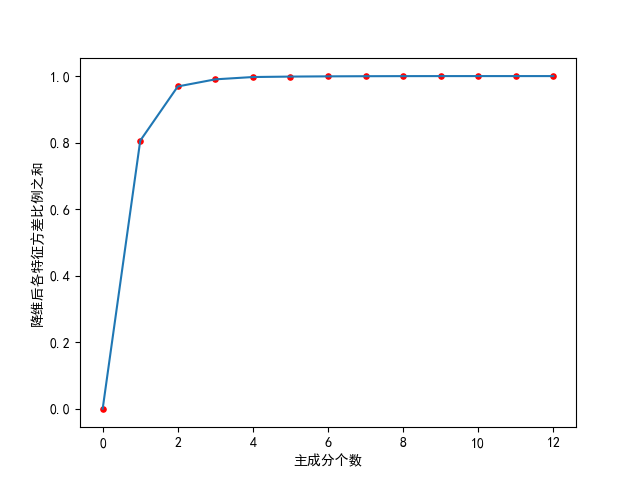
\includegraphics[width=0.35\linewidth]{img/kline-radio.png}
	}
	\subfigure[时间消耗的变化]{
		\label{fig::kline-time}
	    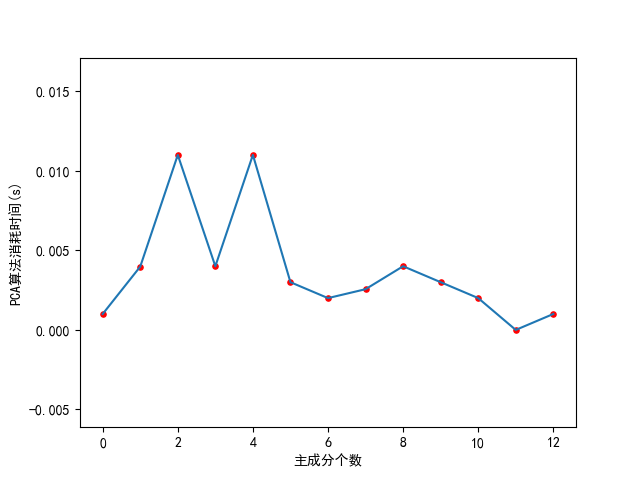
\includegraphics[width=0.35\linewidth]{img/kline-time.png}
	}
	\caption{PCA对于Boston数据集的降维效果}
	\label{fig::kline}
\end{figure}

从图中可以更为明显地看出,主成分的方差占比之和在3个主成分以上时几乎没有提升,且目标主成分个数为3时消耗的时间也处于局部最小值。综合图表数据以及上述分析结果,可以得出:一般应用中,PCA算法在Boston数据集下的最佳主成分个数为3。

\subsection{可视化部分PCA降维效果}

为确认PCA算法的效果,我将主成分个数为1至3的结果可视化(图 \ref{fig:pca_vis})。

\begin{figure}[H]
	\centering
	\subfigure[主成分个数为1]{
		\label{fig::k1}
	    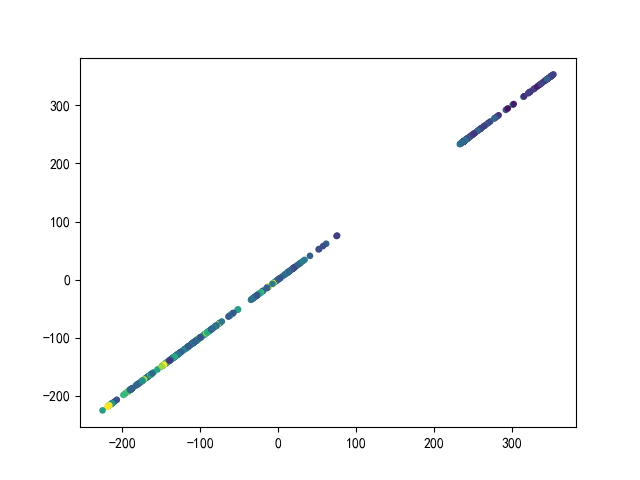
\includegraphics[width=0.3\linewidth]{img/pca-1.png}
	}
	\subfigure[主成分个数为2]{
		\label{fig::k2}
		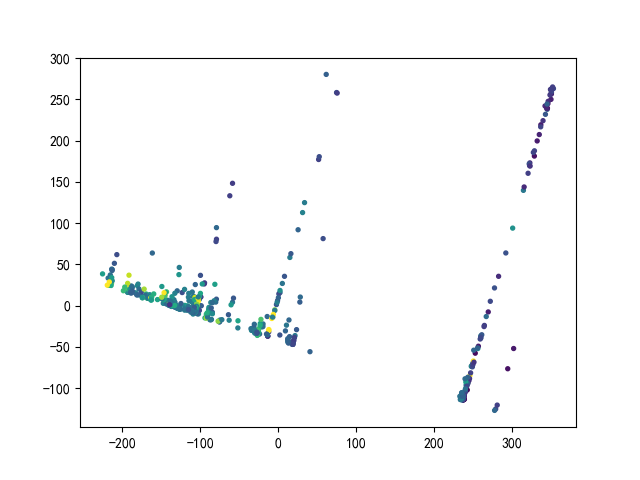
\includegraphics[width=0.3\linewidth]{img/pca-2.png}
	}
	\subfigure[主成分个数为3]{
		\label{fig::k3}
		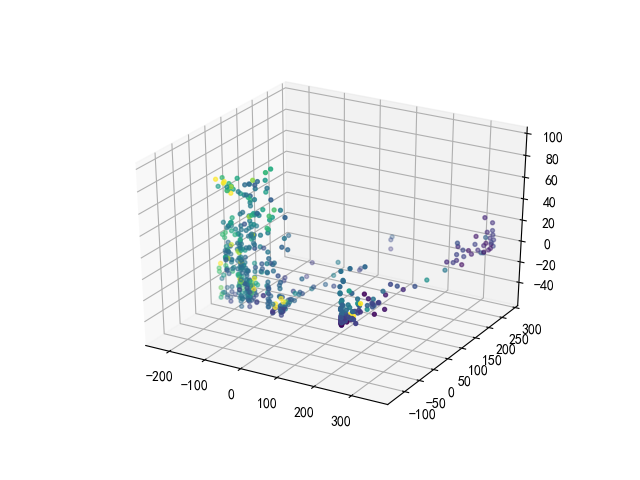
\includegraphics[width=0.3\linewidth]{img/pca-3.png}
	}
	\caption{PCA效果可视化(图中不同点的颜色代表不同的回归目标,即房价,颜色越接近则表示数值越接近)}
	\label{fig:pca_vis}
\end{figure}

容易看出,PCA算法在主成分个数为1时,仅提取出个数为2的部分特征信息(即图 \ref{fig::k2} 右侧的长线);同理,个数为2的结果也仅为图 \ref{fig::k3} 在俯视角度下的信息。因此,上图更为形象地解释了 \ref{sec:pca_res_com} 小节的结果。

同时,我也对主成分个数为3的可视化结果进行了多角度的探索,详细信息可参见附录 \ref{apd:vis3}。

\subsection{PCA在实际应用中的思考}
\label{sec:dis}

本次实验中,我主要根据PCA算法的目标主成分个数执行算法,而在实际应用中,有时也需要直接根据主成分方差占比之和来执行PCA算法,尤其是在特征数极多的情况下(如数万甚至数百万特征)。

Boston数据集属于极小的数据集,仅有506个实例和13个特征,因此执行PCA算法所消耗的时间可忽略不计,且受噪声的影响较大。对于大规模的数据集,如基因芯片数据,实例和特征个数的计量一般以万甚至百万为单位,此时PCA算法消耗的时间即使在40核的并行计算下也将长达数小时或数天之久,直接通过确定目标主成分个数来执行PCA算法显然不现实,一般做法应是直接指定主成分方差占比之和以执行PCA算法。而由于算法消耗的时间和计算资源巨大,对于主成分方差占比之和的选择也应有更全面的考虑。

\newpage
\begin{appendix}
	\section{附录}
	\subsection{Boston数据集特征信息}
	\label{apd:boston_char}
	\begin{table}[H]
		\renewcommand\arraystretch{1.35}
		\caption{Boston数据集特征信息}
		\label{tab:boston_char}
		\centering
		
		\begin{tabular}{c|c|c}
			\centering
			编号 & 特征名 & 特征含义 \\
			\hline
			1 & CRIM & 城镇人均犯罪率 \\
			2 & ZN & 住宅用地超过 25000 sq.ft. 的比例 \\
			3 & INDUS & 城镇非零售商用土地的比例 \\
			4 & CHAS & 查理斯河空变量(如果边界是河流,则为1;否则为0) \\
			5 & NOX & 一氧化氮浓度 \\
			6 & RM & 住宅平均房间数 \\
			7 & AGE & 1940 年之前建成的自用房屋比例 \\
			8 & DIS & 到波士顿五个中心区域的加权距离 \\
			9 & RAD & 辐射性公路的接近指数 \\
			10 & TAX & 每 10000 美元的全值财产税率 \\
			11 & PTRATIO & 城镇师生比例 \\
			12 & B & 1000(Bk-0.63)\^ 2,其中 Bk 指代城镇中黑人的比例 \\
			13 & LSTAT & 人口中地位低下者的比例 \\			
		\end{tabular}
	\end{table}
	
	\subsection{PCA算法在主成分个数为3时的进一步可视化}
	\label{apd:vis3}
	
	\begin{figure}[H]
		\centering
		\subfigure{
		    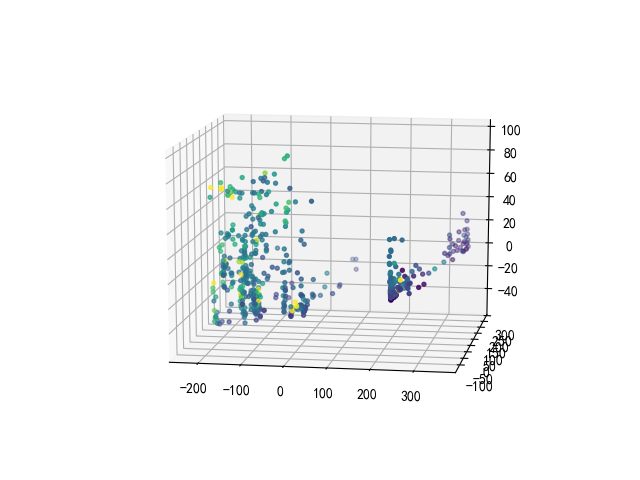
\includegraphics[width=0.3\linewidth]{img/pca-3-0.png}
		}
		\subfigure{
			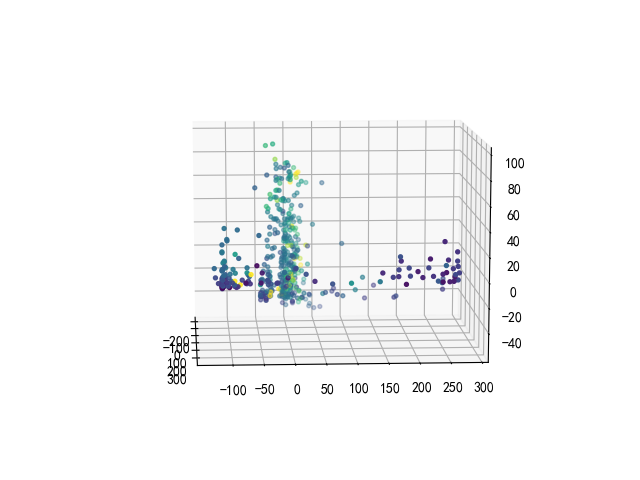
\includegraphics[width=0.3\linewidth]{img/pca-3-1.png}
		}
		\subfigure{
			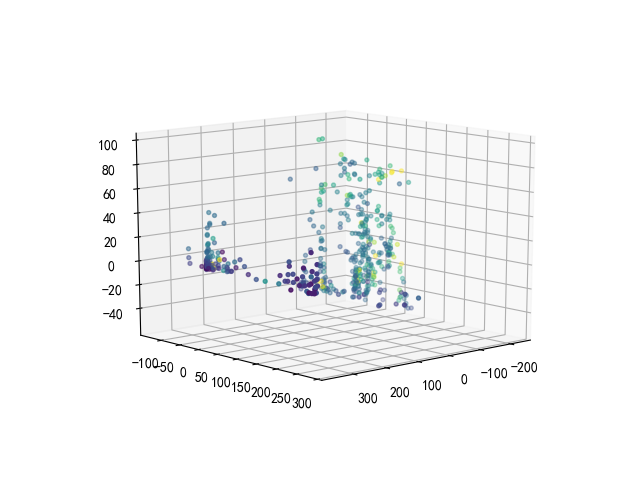
\includegraphics[width=0.3\linewidth]{img/pca-3-2.png}
		}
		\subfigure{
		    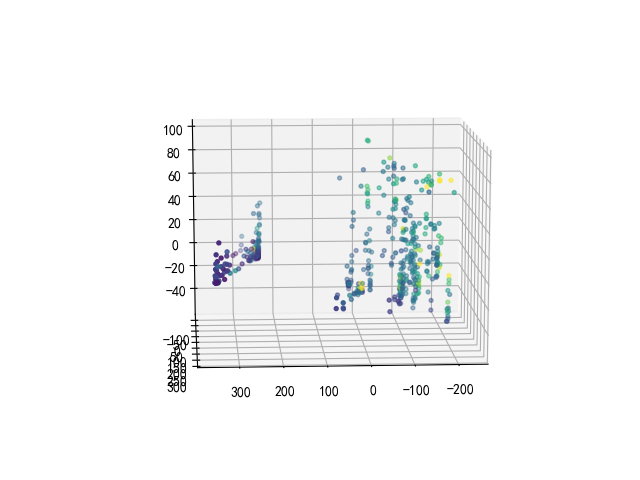
\includegraphics[width=0.3\linewidth]{img/pca-3-3.png}
		}
		\subfigure{
			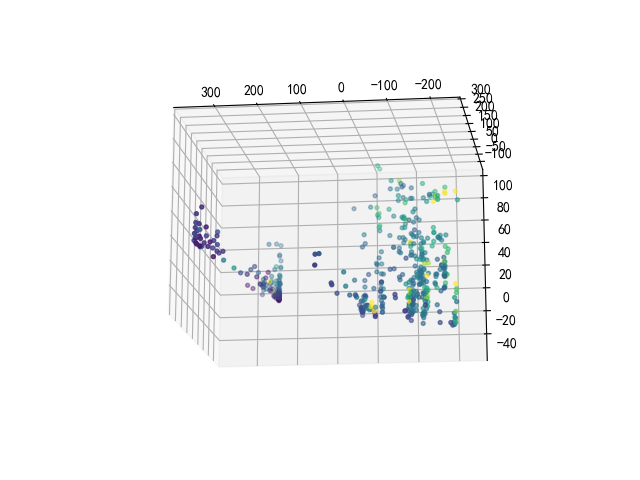
\includegraphics[width=0.3\linewidth]{img/pca-3-4.png}
		}
		\subfigure{
			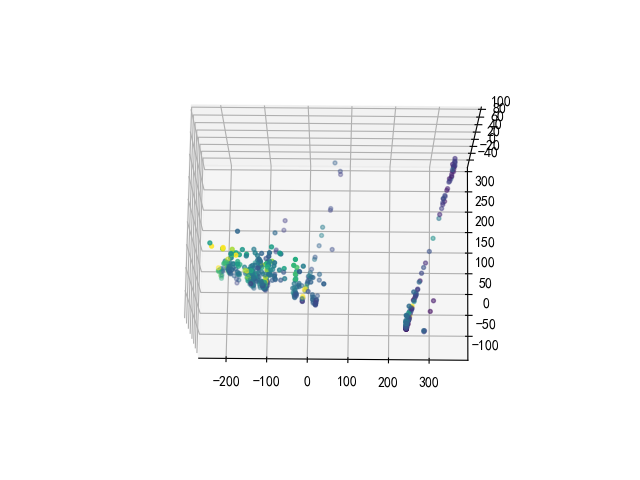
\includegraphics[width=0.3\linewidth]{img/pca-3-5.png}
		}
		\caption{PCA效果进一步可视化(主成分个数为3时)}
		\label{fig::pca_vis3}
	\end{figure}
	
	\subsection{主要代码}
	\label{apd:code}
	
	\begin{lstlisting}[language=Python,
	numbers=left,
	keywordstyle=\color{blue!70},
	frame=shadowbox,
	breaklines=True]
import matplotlib.pyplot as plt
plt.rcParams['font.sans-serif'] = ['SimHei']    # display Chinese
plt.rcParams['axes.unicode_minus'] = False      # display minus sign
from mpl_toolkits.mplot3d import Axes3D
from sklearn import datasets
from sklearn.decomposition import PCA

import os
import time

class bostonAnalyzer(object):
    def __init__(self):
        # load dataset
        self.dataset = datasets.load_boston()
        self.data = self.dataset.data
        self.target = self.dataset.target
        
        # for plot
        self.var = []
        self.t = []

        if not os.path.exists('report/img'):
            os.makedirs('report/img')

    def run(self, vis=False):
        '''
        Run PCA for 1-13 dimensions
        :param vis: True: plot dim 1-3; False: not plot
        '''

        self.var.clear()
        self.t.clear()

        with open('report/result.txt', 'w') as f:
            for i in range(13):
                t = time.time()
                pca_op = PCA(n_components=i)
                pca_res = pca_op.fit_transform(self.data)
                t = time.time() - t

                self.var.append(pca_op.explained_variance_ratio_.sum())
                self.t.append(t)

                # write log
                f.write('###### Dimension %d ######\n' % i)
                f.write(str(pca_res.shape) + '\n')
                f.write(str(pca_op.explained_variance_ratio_) + '\n')
                f.write(str(pca_op.explained_variance_ratio_.sum()) + '\n')
                f.write(str(t) + '\n\n')

                # visualize for debug & plot
                if vis:
                    if i == 1:
                        # plot 1 dimension
                        plt.scatter(pca_res[:, 0], pca_res[:, 0], s=14, c=self.target)
                        plt.savefig('report/img/pca-%d' % i)
                        plt.show()
                    elif i == 2:
                        # plot 2 dimensions
                        plt.scatter(pca_res[:,0], pca_res[:,1], s=8, c=self.target)
                        plt.savefig('report/img/pca-%d' % i)
                        plt.show()
                    elif i == 3:
                        # plot 3 dimensions
                        ax = plt.subplot(projection='3d')
                        ax.scatter(pca_res[:, 0], pca_res[:, 1], pca_res[:, 2], s=8, c=self.target)
                        plt.savefig('report/img/pca-%d' % i)
                        plt.show()

    def show(self):
        '''
        Show the basic info of Boston dataset & plot k-lines
        '''
        print(self.data.shape)
        print(self.target.shape)
        self._k_line_radio()
        self._k_line_time()

    def _k_line_radio(self):
        '''
        Plot k-line of variant radio
        '''
        x = list(range(len(self.var)))
        plt.scatter(x, self.var, s=14, c='r')
        plt.plot(x, self.var)
        plt.xlabel('主成分个数')
        plt.ylabel('降维后各特征方差比例之和')
        plt.savefig('report/img/kline-radio')
        plt.show()

    def _k_line_time(self):
        '''
        Plot k-line of time
        '''
        x = list(range(len(self.t)))
        plt.scatter(x, self.t, s=14, c='r')
        plt.plot(x, self.t)
        plt.xlabel('主成分个数')
        plt.ylabel('PCA算法消耗时间(s)')
        plt.savefig('report/img/kline-time')
        plt.show()

if __name__ == '__main__':
    bA = bostonAnalyzer()
    bA.run(True)
    bA.show()
	\end{lstlisting}
	
\end{appendix}

%========================================================================
\end{document}